% Created 2015-06-21 Dom 18:59
\documentclass[11pt]{article}
\usepackage[utf8]{inputenc}
\usepackage[T1]{fontenc}
\usepackage{fixltx2e}
\usepackage{graphicx}
\usepackage{longtable}
\usepackage{float}
\usepackage{wrapfig}
\usepackage{rotating}
\usepackage[normalem]{ulem}
\usepackage{amsmath}
\usepackage{textcomp}
\usepackage{marvosym}
\usepackage{wasysym}
\usepackage{amssymb}
\usepackage{hyperref}
\tolerance=1000
\usepackage{minted}
\usemintedstyle{perldoc}
\usepackage{tikz}
\usetikzlibrary{decorations.markings}
\tikzstyle{vertex}=[circle, draw, inner sep=0pt, minimum size=7pt]
\providecommand{\vertex}{\node[vertex]}
\usemintedstyle{perldoc}
\usemintedstyle{perldoc}
\newcommand{\tu}{\textunderscore}
\usemintedstyle{perldoc}
\usemintedstyle{perldoc}
\usepackage{tikz,enumerate}
\usetikzlibrary{decorations.markings}
\tikzstyle{vertex}=[circle, draw, inner sep=0pt, minimum size=7pt]
\providecommand{\vertex}{\node[vertex]}
\author{Alice Duarte Scarpa, Bruno Lucian Costa}
\date{2015-06-23}
\title{Trabalho de Estruturas de Dados e Algoritmos}
\hypersetup{
  pdfkeywords={},
  pdfsubject={},
  pdfcreator={Emacs 24.4.1 (Org mode 8.2.10)}}
\begin{document}

\maketitle

\section{Introdução}
\label{sec-1}

Esse relatório é gerado a partir de arquivos org-mode, imagens e
bancos de dados. Todos os arquivos necessários para gerar esse
relatório estão disponíveis no \href{https://github.com/adusca/FGV-EDA}{GitHub}.

O código contido neste relatório é rodado automaticamente toda vez que
o relatório é gerado, e suas saídas estão presentes no próprio
relatório.

Mais detalhes de como gerar o relatório final estão disponíveis no
README do repositório.

\section{Exercício 7.28 (Tardos)}
\label{sec-2}

\subsection{Enunciado}
\label{sec-2-1}

Um grupo de estudantes está escrevendo um módulo para preparar
cronogramas de monitoria. O protótipo inicial deles funciona do
seguinte modo: O cronograma é semanal, de modo que podemos nos focar
em uma única semana.

\begin{itemize}
\item O administrador do curso escolhe um conjunto de $k$
intervalos disjuntos de uma hora de duração $I_1, I_2, \ldots,
      I_k$, nos quais seria possível que monitores dessem suas
monitorias; o cronograma final consistirá de um subconjunto de
alguns (mas geralmente não todos) esses intervalos.
\item Cada monitor então entra com seu horário semanal, informando
as horas em que ele está disponível para monitorias.
\item O administrador então especifica, para parâmetros $a$, $b$ e
$c$, que cada monitor deve dar entre $a$ e $b$ horas de
monitoria por semana, e que um total de $c$ horas de monitoria
deve ser dado semanalmente.
\end{itemize}

O problema é escolher um subconjunto dos horários (intervalos) e
atribuir um monitor a cada um desses horários, respeitando a
disponibilidade dos monitores e as restrições impostas pelo
administrador.


a) Dê um algoritmo polinomial que ou constrói um cronograma
   válido de horas de monitoria (especificando que monitor cobre
   quais horários) ou informa que não há cronograma válido.


b) O algoritmo acima tornou-se popular, e surgiu a vontade de
   controlar também a densidade das monitorias: dado números $d_i$,
   com $i$ entre $1$ e $5$, queremos um cronograma com pelo menos
   $d_i$ horários de monitoria no dia da semana $i$. Dê um
   algoritmo polinomial para resolver o problema com essa restrição
   adicional.


\subsection{Introdução}
\label{sec-2-2}

Queremos modelar esse problema como um problema de fluxo. Para isso
vamos começar com algumas definições de fluxo.

\subsubsection{Definições}
\label{sec-2-2-1}

Uma rede de fluxo é um grafo direcionado $G =
(V, E)$ com as seguintes propriedades:
\begin{itemize}
\item Existe um único vértice \textit{fonte} $s \in V$. Nenhuma aresta entra em $s$.
\item A cada aresta $e$ está associada uma capacidade inteira $c_e$ e
uma demanda $d_e$ tal que $c_e \geq d_e \geq 0$.
\item Existe um único vértice \textit{dreno} $t \in V$. Nenhuma aresta sai de $t$.
\end{itemize}

Um fluxo $f$ de $s$ a $t$ é uma função $f \colon E \to R^+$ que associa a cada
aresta $e$ um valor real não-negativo $f(e)$ tal que:

\begin{enumerate}
\item $\forall e \in E, d_e \leq f(e) \leq c_e$
\item Para todo nó $v \not\in \{s,t\}$:
\[ \sum_{e \text{ chegando em } v} f(e) = \sum_{e \text{ saindo de } v} f(e) \]
\end{enumerate}

$f(e)$ representa o fluxo que vai passar pela aresta $e$. O valor de
um fluxo é o total que parte da fonte $s$, isso é:

\begin{equation}
\label{valor_fluxo} \mathrm{Valor}(f) = \sum_{e \text{ saindo de } s} f(e)
\end{equation}

\subsubsection{Representação}
\label{sec-2-2-2}

Vamos usar uma classe para representar arestas. Uma aresta é
inicializada com as propriedades: vértice de origem, vértice de
destino, capacidade e demanda.

Para facilitar o processamento futuro, vamos adicionar também as
propriedades reversa e original. Reversa aponta para uma outra aresta
reversa à atual, a propriedade original é uma flag indicando se a
aresta pertence à rede original ou não.
\begin{minted}[]{python}
class Aresta():
    def __init__(self, origem, destino, capacidade, demanda):
        self.origem = origem
        self.destino = destino
        self.capacidade = capacidade
        self.demanda = demanda
        self.reversa = None
        self.original = True
\end{minted}

Agora que temos a classe Aresta, vamos usá-la para auxiliar na
representação de uma rede de fluxo também como objeto.

Uma rede de fluxo tem duas propriedades: adjacências, um dicionário
que mapeia cada vértice às arestas que saem dele e fluxo.

O construtor da classe inicializa as duas propriedades como dicionários vazios.

Vamos precisar dos seguintes métodos na nossa classe RedeDeFluxo:

\begin{itemize}
\item \verb~novo_vertice(v)~: Adiciona o vértice v à rede
\item \verb~nova_aresta(origem, destino, capacidade)~: Adiciona uma nova aresta a
rede. Também cria a aresta reversa.
\item \verb~novo_fluxo(f, e)~: Adiciona um fluxo $f$ à aresta $e$
\item \verb~encontra_arestas(v)~: Retorna as arestas que partem do vértice $v$
\item \verb~valor_do_fluxo(fonte)~: Encontra o valor do fluxo, como definido em \eqref{valor_fluxo}.
\end{itemize}

\begin{minted}[]{python}
class RedeDeFluxo():
    def __init__(self):
        self.adj = collections.OrderedDict()
        self.fluxo = {}

    def novo_vertice(self, v):
        self.adj[v] = []

    def nova_aresta(self, origem, destino, capacidade, demanda):
        aresta = Aresta(origem, destino, capacidade, demanda)
        self.adj[origem].append(aresta)

        # Criando a aresta reversa
        aresta_reversa = Aresta(destino, origem, 0, -demanda)
        self.adj[destino].append(aresta_reversa)
        aresta_reversa.original = False

        # Marcando aresta e aresta_reversa como reversas uma da outra
        aresta.reversa = aresta_reversa
        aresta_reversa.reversa = aresta

    def novo_fluxo(self, e, f):
        self.fluxo[e] = f

    def encontra_arestas(self, v):
        return self.adj[v]

    def valor_do_fluxo(self, fonte):
        valor = 0
        for aresta in self.encontra_arestas(fonte):
            valor += self.fluxo[aresta]
        return valor
\end{minted}

\subsection{Modelando o problema com fluxos\label{modelagem_fluxo}}
\label{sec-2-3}

Os dois itens do problema podem ser reduzidos a encontrar um fluxo
válido em uma rede usando construções semelhantes.

Para o item a), construimos o grafo da seguinte forma:

\begin{itemize}
\item Criamos um vértice $s$ representando a fonte e um vértice $t$
  representando o dreno
\item Para cada intervalo $I_i \in I_1, I_2, \ldots, I_k$ escolhido pelo
administrador, criamos um vértice $I_i$ e uma aresta $(s, I_i)$
capacidade 1 e demanda 0
\item Para cada monitor $T_i \in T_1, T_2, \ldots, T_m$ criamos um vértice
$T_i$. Se o monitor está disponível para dar monitoria no intervalo
$I_j$ criamos uma aresta de $(I_j, T_i)$ de demanda 0 e
capacidade 1. Para cada monitor também criamos uma aresta
$(T_i, t)$ de demanda $a$ e capacidade $b$.
\item Para garantir que a solução final terá exatamente $c$ horas de
monitoria, criamos uma nova fonte $s'$ e uma aresta $(s', s)$
com demanda e capacidade $c$.
\end{itemize}

Para construir uma atribuição de intervalos válida a partir de um
fluxo, é suficiente atribuir um intervalo a um monitor se a aresta que
liga o intervalo ao monitor tem fluxo 1.  As condições de capacidade e
demanda da rede garantem que um intervalo é atribuído a no máximo um
monitor, que cada monitor recebe apenas intervalos compatíveis com ele
e que as restrições no número de hora são satisfeitas.

Reciprocamente, para toda atribuição de intervalos válida, podemos
construir um fluxo passando uma unidade de fluxo pelo caminho $(s', s, I,
T, t)$ para cada par $(I, T)$ de intervalo e monitor correspondente. A
validade da atribuição implica imediatamente que as condições de
demanda e capacidade são atendidas.

O caso com 3 intervalos e 2 monitores (A e B) em que o monitor A está
disponível nos intervalos 1 e 2 e o monitor B está disponível nos
horários 1 e 3 está representado abaixo. Os rótulos
das arestas são da forma demanda/capacidade. As
arestas sem rótulo tem demanda 0 e capacidade 1.


\[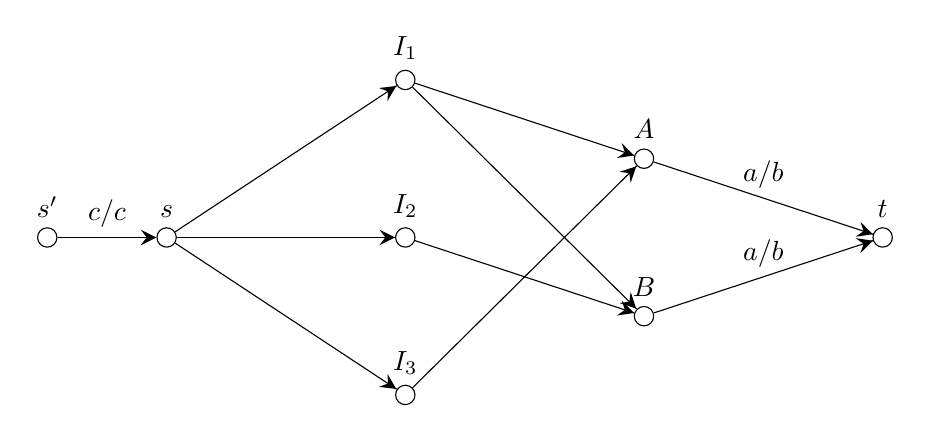
\begin{tikzpicture}[x=0.25\textwidth,
    every edge/.style={
        draw,
        postaction={decorate,
                    decoration={markings,mark=at position 1 with {\arrow[line width = 0.5mm]{stealth}}}
                   }
        }
]
\vertex (fonte') at (0,3) [label=above:$s$] {};
\vertex (fonte) at (-0.5,3) [label=above:$s'$] {};
\vertex (I1) at (1,5) [label=above:$I_1$] {};
\vertex (I2) at (1,3) [label=above:$I_2$] {};
\vertex (I3) at (1,1) [label=above:$I_3$] {};
\vertex (A) at (2,4) [label=above:$A$] {};
\vertex (B) at (2,2) [label=above:$B$] {};
\vertex (dreno) at (3,3) [label=above:$t$] {};
\path
(fonte) edge node [above] {$c/c$} (fonte')
(fonte') edge (I1)
(fonte') edge (I2)
(fonte') edge (I3)
(I1) edge (A)
(I1) edge (B)
(I2) edge (B)
(I3) edge (A)
(A) edge node [above] {$a/b$} (dreno)
(B) edge node [above] {$a/b$} (dreno)
;
\end{tikzpicture}\]

A única diferença na construção do item b é que, ao invés de ligarmos
$s$ diretamente aos intervalos de monitoria, ligamos $s$ a cada dia da
semana i com demanda $d_i$ e capacidade $c$ e depois
criamos uma aresta com demanda 0 e capacidade 1 de
cada dia da semana para os intervalos que são naquele dia.

Abaixo está o mesmo exemplo do item a) com dias da semana. Para deixar
a visualização mais simples estamos colocando aqui apenas dois dias da
semana.

\[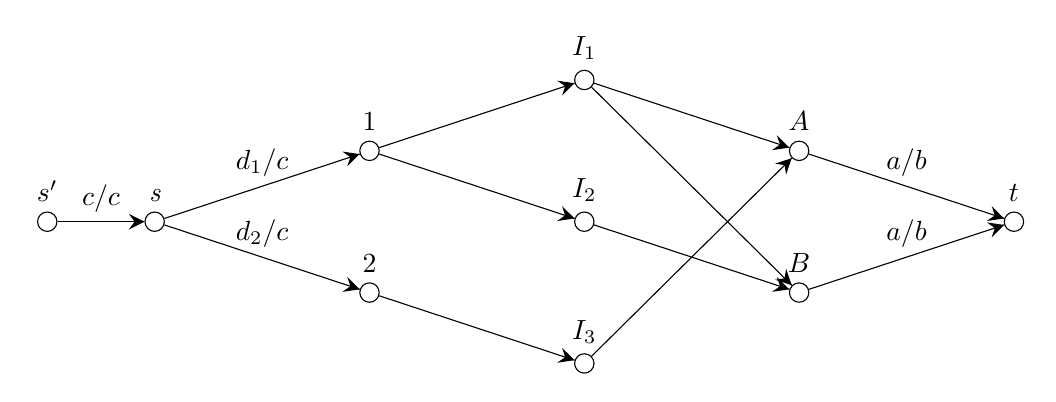
\begin{tikzpicture}[x=0.25\textwidth, scale=0.9,
    every edge/.style={
        draw,
        postaction={decorate,
                    decoration={markings,mark=at position 1 with {\arrow[line width = 0.5mm]{stealth}}}
                   }
        }
]
\vertex (fonte') at (0,3) [label=above:$\textit{s}$] {};
\vertex (fonte) at (-0.5,3) [label=above:$s'$] {};
\vertex (1) at (1, 4) [label=above:$1$] {};
\vertex (2) at (1, 2) [label=above:$2$] {};
\vertex (I1) at (2,5) [label=above:$I_1$] {};
\vertex (I2) at (2,3) [label=above:$I_2$] {};
\vertex (I3) at (2,1) [label=above:$I_3$] {};
\vertex (A) at (3,4) [label=above:$A$] {};
\vertex (B) at (3,2) [label=above:$B$] {};
\vertex (dreno) at (4,3) [label=above:$t$] {};
\path
(fonte) edge node [above] {$c/c$} (fonte')
(fonte') edge node [above] {$d_1/c$} (1)
(fonte') edge node [above] {$d_2/c$} (2)
(1) edge (I1)
(1) edge (I2)
(2) edge (I3)
(I1) edge (A)
(I1) edge (B)
(I2) edge (B)
(I3) edge (A)
(A) edge node [above] {$a/b$} (dreno)
(B) edge node [above] {$a/b$} (dreno)
;
\end{tikzpicture}\]

\subsection{Implementação}
\label{sec-2-4}

\subsubsection{Fluxo máximo}
\label{sec-2-4-1}

Vamos começar estudando o problema de encontrar o fluxo máximo de uma
rede $G$ em que $d_e = 0 \; \forall e \in E$ $f$. Vamos implementar aqui o
algoritmo de Ford-Fulkerson para resolver esse problema.

O algoritmo tem 2 partes:

\begin{enumerate}
\item Dado um caminho $P$ e partindo de um fluxo inicial $f$, obter um
novo fluxo $f'$ expandindo $f$ em $P$
\item Partindo do fluxo $f(e)$ = 0, expandir o fluxo enquanto for possível
\end{enumerate}


\begin{itemize}
\item Primeira parte:
\end{itemize}

Queremos expandir o fluxo $f$ em $P$. Mais precisamente, queremos
mudar o valor do fluxo somando $x$ ao valor de $f(e)$ para toda aresta
$e$ que está no caminho $P$.

O gargalo de um caminho $P$ (com relação a um fluxo $f$) é o maior
valor de $x$ tal que $f(e) + x \leq c_e$ para toda aresta $e \in
P$. Essa última condição significa que o fluxo

\[ f'(e) = \begin{cases}f(e)&\text{ se } e \not\in P \\
                        f(e) + x&\text{ se } e \in P\end{cases} \]

ainda satisfaz as restrições de capacidade. O código abaixo computa
tal valor de $x$.
\begin{minted}[]{python}
def encontra_gargalo(self, caminho):
    residuos = []
    for aresta in caminho:
        residuos.append(aresta.capacidade - self.fluxo[aresta])
    return min(residuos)
\end{minted}

Como descrito acima, expandir o caminho é somar $x$ ao valor de $f(e)$
para cada aresta do caminho. Precisamos atualizar também as arestas
reversas, pois elas precisam satisfazer a propriedade $f(e) =
-f(e.reversa)$.
\begin{minted}[]{python}
def expande_caminho(self, caminho):
    gargalo = self.encontra_gargalo(caminho)
    for aresta in caminho:
        self.fluxo[aresta] += gargalo
        self.fluxo[aresta.reversa] -= gargalo
\end{minted}

Pela definição de gargalo, a operação de expandir $P$ gera um fluxo
válido. Se garantirmos que $c_e - f(e)$ é positivo para toda $e \in
P$, então o gargalo também será positivo, de modo que o fluxo $f'$
obtido terá valor maior que o anterior.

Tendo a restrição acima em mente, iremos fazer uma DFS no grafo,
usando apenas as arestas que possuem $c_e - f(e)$ (chamaremos esse
valor de \verb~residuo~) positivo.

Mais precisamente, a função abaixo recebe um caminho parcialmente
construído da fonte até \verb~v~ na variável \verb~caminho~ e recursivamente
encontra uma maneira de chegar em dreno a partir de \verb~v~ usando apenas
vértices não explorados. Se um caminho de \verb~v~ a dreno não existir, a
função não retorna um valor (isto é, retorna \verb~None~).

\begin{minted}[]{python}
def encontra_caminho(self, v, dreno, caminho, visitados):
    if v == dreno:
        return caminho

    visitados.add(v)

    for aresta in self.encontra_arestas(v):
        residuo = aresta.capacidade - self.fluxo[aresta]
        if residuo > 0 and aresta.destino not in visitados:
            resp = self.encontra_caminho(aresta.destino,
                                         dreno,
                                         caminho + [aresta],
                                         visitados)
            if resp != None:
                return resp
\end{minted}

Como só chamamos a função com primeiro parâmetro igual a \verb~w~ quando
\verb~w~ não está no conjunto de vértices visitados e \verb~w~ é imediatamente
colocado em tal conjunto depois da chamada, chamamos a função uma
única vez por vértice. Como a função demora tempo proporcional ao
número de arestas que saem do vértice em questão, o tempo total gasto
em todas as chamadas da função é $O(|V| + |E|)$.

Para as outras funções, note que um caminho tem no máximo $|V|$
vértices, e portanto as funções \verb~encontra_gargalo~ e \verb~expande_caminho~
têm complexidade $O(|V|)$.

Para a parte 2, vamos precisar criar um fluxo $f$ com $f(e) = 0$ para
toda aresta $e$. Podemos fazer isso utilizando o seguinte método na
classe RedeDeFluxo():
\begin{minted}[]{python}
def cria_fluxo_inicial(self):
    for vertice, arestas in self.adj.iteritems():
        for aresta in arestas:
            self.fluxo[aresta] = 0
\end{minted}

Com todas as funções auxiliares prontas, podemos finalmente definir a
função que encontra o fluxo máximo, repetidamente aumentando o fluxo
como descrito na parte 1:
\begin{minted}[]{python}
def fluxo_maximo(self, fonte, dreno):
    self.cria_fluxo_inicial()

    caminho = self.encontra_caminho(fonte, dreno, [], set())
    while caminho is not None:
        self.expande_caminho(caminho)
        caminho = self.encontra_caminho(fonte, dreno, [], set())
    return self.valor_do_fluxo(fonte)
\end{minted}

Como o fluxo aumenta em pelo menos uma unidade por iteração e o custo
de uma iteração é $O(|V| + |E|)$, a complexidade total do algoritmo é
$O((|V|+|E|)F)$, onde $F$ é o fluxo máximo possível na rede. No caso
do exercício, $F$ é no máximo o número de intervalos e portanto
polinomial no tamanho da entrada.

\subsubsection{Fluxo válido com demandas não-nulas}
\label{sec-2-4-2}

O nosso objetivo é encontrar um fluxo válido $f$ para uma rede $G =
(V, E)$ no caso em que as demandas são positivas.

Vamos construir uma rede $G' = (V', E')$ com um valor associado $d$
tal que $d_e = 0 \; \forall e \in E'$ de tal forma que um fluxo válido
para $G$ existe se e somente se o valor do fluxo máximo em $G'$ é
$d$. Em caso afirmativo, podemos construir um fluxo válido $f$ para
$G$ rapidamente a partir de qualquer fluxo máximo $f'$ de $G'$.

Construimos $G'$ da seguinte forma:

\begin{itemize}
\item Criamos um vértice em $G'$ para cada vértice $G$
\item Adicionamos uma fonte adicional $F$ e um dreno adicional $D$ a $G'$
\item Definimos o saldo de cada vértice $v \in V$ como: \[
  \textrm{saldo}(v) = \sum_{e \text{ saindo de }v}d_e - \sum_{e \text{
  chegando em }v}d_e \]
\item Se $\mathrm{saldo}(v) > 0$ adicionamos uma aresta $(v, D,
  \mathrm{saldo}(v), 0)$ a $G'$
\item Se $\mathrm{saldo}(v) < 0$ adicionamos uma aresta $(F, v,
  -\mathrm{saldo}(v), 0)$ a $G'$
\item Para cada aresta $e = (\mathrm{origem, destino, capacidade,
  demanda}) \in E$, crie uma aresta $e' = (\mathrm{origem, destino,
  capacidade - demanda, 0})$ em $G'$
\end{itemize}

Codificando a construção acima:
\begin{minted}[]{python}
def cria_rede_com_demandas_nulas(G):
    G_ = RedeDeFluxo()
    G_.novo_vertice('F')
    G_.novo_vertice('D')
    d = 0

    for vertice, arestas in G.adj.iteritems():
        G_.novo_vertice(vertice)
        saldo = sum(e.demanda for e in arestas)
        if saldo > 0:
            G_.nova_aresta(vertice, 'D', saldo, 0)
            d += saldo
        elif saldo < 0:
            G_.nova_aresta('F', vertice, -saldo, 0)

    for arestas in G.adj.values():
        for a in arestas:
             if a.original:
                 G_.nova_aresta(a.origem,
                                a.destino,
                                a.capacidade - a.demanda,
                                0)
    return G_, d
\end{minted}

\subsection{Rodando o algoritmo}
\label{sec-2-5}

\subsubsection{Item A}
\label{sec-2-5-1}
A seguinte tabela mostra a disponibilidade dos monitores nos horários
escolhidos pelo administrador:

\begin{center}
\begin{tabular}{lccccccccc}
 & Ana & Bia & Caio & Davi & Edu & Felipe & Gabi & Hugo & Isa\\
Seg 10h &  &  &  & x &  &  &  &  & \\
Seg 14h &  &  &  &  &  & x & x & x & x\\
Seg 21h & x &  &  & x &  &  &  &  & \\
Ter 10h & x & x &  & x &  &  &  &  & \\
Ter 16h &  &  & x &  &  &  &  &  & \\
Ter 20h &  &  &  &  &  &  & x &  & x\\
Qua 9h &  &  &  &  &  & x &  &  & \\
Qua 17h &  &  & x &  &  &  &  &  & \\
Qua 19h &  &  &  &  &  &  &  & x & \\
Qui 7h &  & x &  &  &  & x &  &  & \\
Qui 13h &  &  &  &  &  &  & x &  & \\
Qui 19h &  & x &  &  & x &  &  & x & \\
Sex 7h &  &  & x &  & x &  &  &  & \\
Sex 11h & x &  &  &  & x &  &  &  & x\\
Sex 21h &  &  & x &  &  & x &  &  & x\\
\end{tabular}
\end{center}
As outras regras para monitoria estão na tabela abaixo:

\begin{center}
\begin{tabular}{lr}
Min de horas por monitor & 1\\
Max de horas por monitor & 3\\
Horas de monitoria & 10\\
\end{tabular}
\end{center}

Podemos carregar as informações das tabelas para criar uma rede como
descrita no final da Seção \ref{modelagem_fluxo}.
\begin{minted}[]{python}
# Lendo a tabela de disponibilidade
intervalos = collections.OrderedDict()
monitores = horarios[0][1:]

for disponibilidade in horarios[1:]:
    intervalos[disponibilidade[0]] = []
    for i, slot in enumerate(disponibilidade[1:]):
        if slot != '':
            intervalos[disponibilidade[0]].append(monitores[i])
\end{minted}

Lendo a tabela de regras
\begin{minted}[]{python}
min_horas = regras[0][1]
max_horas = regras[1][1]
total_horas = regras[2][1]
\end{minted}

Criando uma rede para o problema com os dados fornecidos

\begin{minted}[]{python}
def cria_rede(intervalos, monitores, min_horas, max_horas, total_horas):
    G = RedeDeFluxo()
    G.novo_vertice('Fonte')
    G.novo_vertice('Dreno')
    G.nova_aresta('Dreno', 'Fonte', total_horas, total_horas)

    # Criando um vertice para cada monitor e ligando esse vertice
    # ao dreno
    for monitor in monitores:
        G.novo_vertice(monitor)
        G.nova_aresta(monitor, 'Dreno', max_horas, min_horas)

    for intervalo, monitores_disponiveis in intervalos.iteritems():
        # Criando um vertice para cada intervalo e conectando a
        # fonte a cada um dos intervalos
        G.novo_vertice(intervalo)
        G.nova_aresta('Fonte', intervalo, 1, 0)

        # Conectando o intervalo a cada monitor disponivel nele
        for monitor in monitores_disponiveis:
            G.nova_aresta(intervalo, monitor, 1, 0)

    return G
\end{minted}

Agora é só rodar o algoritmo com o grafo obtido:
\begin{minted}[]{python}
G = cria_rede(intervalos, monitores, min_horas, max_horas, total_horas)
G_, d = cria_rede_com_demandas_nulas(G)
fluxo = G_.fluxo_maximo('F', 'D')
if fluxo == d:
    tabela_de_monitores = []
    for horario in intervalos:
        for w in G_.adj[horario]:
            if G_.fluxo[w] == 1:
                tabela_de_monitores.append([w.origem, w.destino])
    return tabela_de_monitores
else:
    return 'Impossivel'
\end{minted}

No final, obtemos ou 'Impossível' se não existir um horário compatível
ou uma tabela com um horário que atende a todas as restrições.

Para a tabela acima:
\begin{center}
\begin{tabular}{ll}
Seg 10h & Davi\\
Seg 14h & Gabi\\
Seg 21h & Ana\\
Ter 10h & Bia\\
Ter 16h & Caio\\
Ter 20h & Isa\\
Qua 9h & Felipe\\
Qua 17h & Caio\\
Qua 19h & Hugo\\
Qui 19h & Edu\\
\end{tabular}
\end{center}

\subsubsection{Item B}
\label{sec-2-5-2}

No item b, além de todas as restrições do item a, há também a
restrição de mínimo de horas por dia da semana.

Vamos expressar a nova restrição com uma tabela:

\begin{center}
\begin{tabular}{lr}
Seg & 1\\
Ter & 1\\
Qua & 2\\
Qui & 1\\
Sex & 1\\
\end{tabular}
\end{center}

Parsear a nova tabela é simples:
\begin{minted}[]{python}
minimo_por_dia = {}
for dia in min_por_dia:
    minimo_por_dia[dia[0]] = dia[1]
\end{minted}

A única função que precisamos alterar do item a é a função
\verb~cria_rede~, que agora tem que lidar com a construção mencionada na
Seção \ref{modelagem_fluxo}.

\begin{minted}[]{python}
def cria_rede(intervalos, monitores, min_horas,
              max_horas, total_horas, minimo_por_dia):
    G = RedeDeFluxo()
    G.novo_vertice('Fonte')
    G.novo_vertice('Dreno')
    G.nova_aresta('Dreno', 'Fonte', total_horas, total_horas)

    # Criando um vertice para cada monitor e ligando esse vertice
    # ao dreno
    for monitor in monitores:
        G.novo_vertice(monitor)
        G.nova_aresta(monitor, 'Dreno', max_horas, min_horas)

    # Criando um vertice para cada dia e uma aresta da Fonte
    # ao dia com demanda igual ao minimo de horas de monitoria
    # para aquele dia e capacidade suficientemente grande
    # (vamos usar o total de horas)
    dias = minimo_por_dia.keys()
    for dia in dias:
        G.novo_vertice(dia)
        G.nova_aresta('Fonte', dia, total_horas, minimo_por_dia[dia])

    for intervalo, monitores_disponiveis in intervalos.iteritems():
        # Encontrando o dia do intervalo
        for dia in dias:
            if intervalo.startswith(dia):
                dia_do_intervalo = dia

        # Criando um vertice para cada intervalo e conectando o
        # dia do intervalo a cada um dos intervalos
        G.novo_vertice(intervalo)
        G.nova_aresta(dia_do_intervalo, intervalo, 1, 0)

        # Conectando o intervalo a cada monitor disponivel nele
        for monitor in monitores_disponiveis:
            G.nova_aresta(intervalo, monitor, 1, 0)

    return G
\end{minted}

\begin{center}
\begin{tabular}{ll}
Seg 10h & Davi\\
Seg 14h & Isa\\
Seg 21h & Ana\\
Ter 10h & Bia\\
Ter 16h & Caio\\
Qua 9h & Felipe\\
Qua 17h & Caio\\
Qua 19h & Hugo\\
Qui 13h & Gabi\\
Sex 7h & Edu\\
\end{tabular}
\end{center}

\section{Exercício 6.3 (Papadimitriou)}
\label{sec-3}

\subsection{Enunciado}
\label{sec-3-1}

O Yuckdonald's está considerando abrir uma cadeia de restaurantes em
Quaint Valley Highway (QVG). Os $n$ locais possíveis estão em uma
linha reta, e as distâncias desses locais até o começo da QVG são, em
milhas e em ordem crescente, $m_1, m_2, \ldots, m_n$. As restrições
são as seguintes:

\begin{itemize}
\item Em cada local, o Yuckdonald's pode abrir no máximo um
restaurante. O lucro esperado ao abrir um restaurante no local
$i$ é $p_i$, onde $p_i > 0$ e $i = 1, 2, \ldots, n$.
\item Quaisquer dois restaurantes devem estar a pelo menos $k$
  milhas de distância, onde $k$ é um inteiro positivo.
\end{itemize}

Dê um algoritmo eficiente para computar o maior lucro total
esperado, sujeito às restrições acima.

\section{Exercício 6.30 (Papadimitriou)}
\label{sec-4}

\subsection{Enunciado}
\label{sec-4-1}

\textit{Reconstruindo árvores filogenéticas pelo método da máxima parcimônia}

Uma árvore filogenética é uma árvore em que as folhas são espécies
diferentes, cuja raiz é o ancestral comum de tais espécies e cujos
galhos representam eventos de especiação.

Queremos achar:

\begin{itemize}
\item Uma árvore (binária) evolucionária com as espécies dadas
\item Para cada nó interno uma string de comprimento $k$ com a
sequência genética daquele ancestral.
\end{itemize}


Dada uma árvore acompanhada de uma string $s(u) \in \{A, C, G, T\}^k$ para
cada nó $u \in V(T)$, podemos atribuir uma nota usando o método da
máxima parcimônia, que diz que menos mutações são mais prováveis:
\[ \mathrm{nota}(T) = \sum_{(u,v) \in E(T)} (\text{número de posições em que }s(u)\text{ e }s(v)\text{ diferem}). \]

Achar a árvore com nota mais baixa é um problema difícil. Aqui vamos
considerar um problema menor: Dada a estrutura da árvore, achar as
sequências genéticas $s(u)$ para os nós internos que dêem a nota mais
baixa.

Um exemplo com $k = 4$ e $n = 5$:

\href{http://github.com/adusca/FGV-EDA/6_30/tree.png}{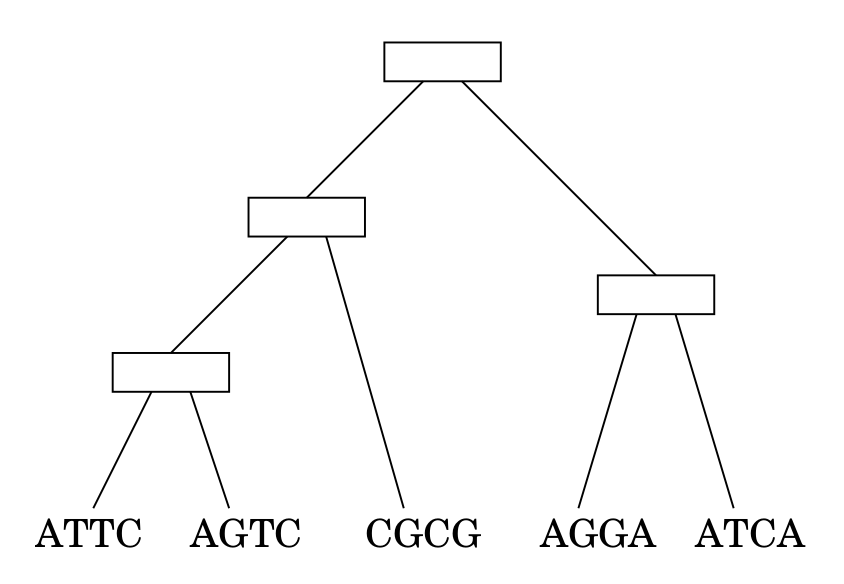
\includegraphics[width=.9\linewidth]{tree.png}}

\begin{enumerate}
\item Ache uma reconstrução para o exemplo seguindo o método da
máxima parcimônia.
\item Dê um algoritmo eficiente para essa tarefa.
\end{enumerate}

\subsection{Solução}
\label{sec-4-2}

A nota final de uma árvore é a soma da nota de cada letra. Podemos
calcular a resposta para cada letra independentemente e depois
concatenar as respostas para obter a árvore final.

Nós vamos usar um algoritmo de programação dinâmica para encontrar o
valor das folhas intermediárias em uma árvore $P$ em que cada folha
tem valor A, G, T ou C. Como em dados reais de bioinformática é muito
comum representar uma deleção como o carácter extra '-', também vamos
suportar essa opção na nossa solução.

Vamos representar a nossa árvore como um objeto:
\begin{minted}[]{python}
class Arvore:
    def __init__(self, pai):
        self.filhos = []
        self.valor = ""
        self.pai = pai
        self.nome = ""
\end{minted}

Vamos computar $melhor\tu nota[v, \ell]$ como a melhor maneira de
preencher os nós da sub-árvore enraizada em $v$, dado que o pai de $v$
tem valor $\ell$. Também preencheremos $melhor \tu letra[v, \ell]$ com um valor possível
de uma configuração otimal. Guardaremos tais valores em dicionários.

\begin{minted}[]{python}
melhor_nota = {}
melhor_letra = {}
\end{minted}

Vamos computar $melhor \tu nota$ de baixo para cima. Então, o caso base
para esse algoritmo é a resposta para as folhas, isto é, $melhor\tu nota[\mathrm{folha}, \ell]$.

Uma sub-árvore que contém apenas uma folha e seu pai vai ter
nota 0 se a folha e o pai tiverem ambos o mesmo valor (A,
G, T ou C) ou nota 1 se os dois tiverem valores diferentes:

\[melhor \tu nota[\textit{folha}, \ell] = \begin{cases}0 \text{ se } \textit{folha}.valor = \ell \\
                                                       1 \text{ caso contrário}\end{cases}\]

Além disso, não temos escolha para o valor otimal:
\[ melhor \tu valor[\textit{folha}, \ell] = \textit{folha}.valor \]

Tendo o caso base, podemos computar $melhor \tu nota[v, \ell]$
assumindo que $melhor \tu nota[w, \ell]$ já foi computado para todo
$w$ filho de $v$ e $\ell \in \{A, G, T, C\}$.

Dado que o pai de $v$ tem valor $\ell$, a melhor nota para a
sub-árvore enraizada em $v$ quando o valor de $v$ é igual a $m$ é:
\[ [\ell \neq m] + \sum_{w \text{ filho de }v} melhor \tu nota[w, m]\]

Onde \[[\ell \neq m] =  \begin{cases} 0 \text{ se } m = \ell \\
                                      1 \text{ caso contrário}\end{cases}\]

Queremos escolher um valor $m \in \{A, G, T, C\}$ para $v$
que minimize a nota final da sub-árvore. Então:
\[melhor \tu nota[v, \ell] = \min_{m \in \{A, G, T, C\}} \left([\ell
\neq m] + \sum_{w \text{ filho de }v} melhor \tu nota[w, m]\right)\]

e $melhor\tu letra[v, \ell]$ é um valor de $m$ que atinge o mínimo
acima.

Implementando o que descrevemos recursivamente, obtemos a seguinte
função:
\begin{minted}[]{python}
def calcula_melhor_nota(v, l):
    if (v, l) in melhor_nota:
        return melhor_nota[v, l]

    if not v.filhos:
        melhor_nota[v, l] = 1 if l != v.valor else 0
        melhor_letra[v, l] = v.valor
        return melhor_nota[v, l]

    melhor_nota[v, l] = 100000

    for m in ['A', 'G', 'T', 'C', '-']:
        nota_atual = sum(calcula_melhor_nota(w, m) for w in v.filhos)
        if m != l:
            nota_atual += 1

        if nota_atual < melhor_nota[v, l]:
            melhor_nota[v, l] = nota_atual
            melhor_letra[v, l] = m

    return melhor_nota[v, l]
\end{minted}

Sabendo calcular $melhor \tu nota[v, \ell]$ para todos os vértices
exceto a raiz podemos encontrar a nota da árvore como o mínimo entre
os possíveis valores para a raiz:
\[ \min_{\ell \in \{A, G, T, C\}} \sum_{v \text{ filho da raiz}}
melhor \tu nota[v, \ell]\]

Um valor ótimo para a raiz é um valor de $\ell$ para o qual o mínimo
acima é atingido.


Podemos agora preencher toda a árvore:
\begin{minted}[]{python}
def preenche_tudo(raiz):
    melhor_nota_raiz = 100000
    for l in ['A', 'G', 'T', 'C', '-']:
        nota_atual_raiz = sum(calcula_melhor_nota(w, l) for w in raiz.filhos)

        if nota_atual_raiz < melhor_nota_raiz:
            raiz.valor = l
            melhor_nota_raiz = nota_atual_raiz

    def preenche_dado_pai(v):
        v.valor = melhor_letra[v, v.pai.valor]
        for w in v.filhos:
            preenche_dado_pai(w)

    for w in raiz.filhos:
        preenche_dado_pai(w)

    return raiz, melhor_nota_raiz
\end{minted}

\subsection{Rodando o algoritmo}
\label{sec-4-3}

\subsubsection{Formato Newick}
\label{sec-4-3-1}

Um formato muito usado para árvores em bioinformática é o formato
Newick. Assim como as $s$-expressions do LISP, ele usa o fato de que
parênteses podem ser usados para especificar uma árvore.

\begin{enumerate}
\item Parseando o formato Newick
\label{sec-4-3-1-1}

O primeiro passo é notar que (gato, rato) é equivalente a
(gato)(rato), então podemos transformar uma estrutura com vírgulas
em uma estrutura que só contém parênteses.

Depois construimos a árvore adicionando vértices novos conforme os
parênteses.
\begin{minted}[]{python}
def parseia_newick(string):
    string = string.replace(',', ')(').replace(';', '')

    em_construcao = collections.deque()
    em_construcao.append(Arvore(None))

    for ch in string:
        if ch == '(':
            pai_atual = em_construcao[-1]
            filho_novo = Arvore(pai_atual)
            pai_atual.filhos.append(filho_novo)
            em_construcao.append(filho_novo)
        elif ch == ')':
            em_construcao.pop()
        else:
            em_construcao[-1].nome += ch

    assert len(em_construcao) == 1
    return em_construcao[0]
\end{minted}
\end{enumerate}

\subsubsection{Formato FASTA}
\label{sec-4-3-2}

Outro formato muito comum em bioinformática é o formato FASTA. É um
formato bem simples:

\begin{verbatim}
>Nome
Sequência de DNA
que pode estar em
várias linhas
\end{verbatim}

Vamos escrever uma função para converter dados no formato FASTA em um
dicionário:
\begin{minted}[]{python}
def fasta_para_dict(linhas):
    nome = ""
    dna = ""
    saida = {}

    for linha_atual in linhas:
        if linha_atual[0] == ">":
            if nome != "":
                saida[nome] = dna
                dna = ""
            nome = linha_atual[1:]
        else:
            dna += linha_atual

    saida[nome] = dna

    return saida
\end{minted}

\subsubsection{Separando e concatenando árvores}
\label{sec-4-3-3}

As árvores no nosso algoritmo só tem uma letra por nó, mas nós
recebemos apenas uma árvore com toda a string de DNA.

Precisamos de um método para capaz de criar uma árvore para cada
carácter. A seguinte DFS cria a árvore das $i$-ésimas letras:
\begin{minted}[]{python}
def separa_arvore(indice, origem):
    copia_origem = Arvore(None)
    copia_origem.nome = origem.nome

    if len(origem.valor):
        copia_origem.valor = origem.valor[indice]

    for filho in origem.filhos:
        copia_filho = separa_arvore(indice, filho)
        copia_filho.pai = copia_origem
        copia_origem.filhos.append(copia_filho)

    return copia_origem
\end{minted}


Depois de rodar o algoritmo, vamos querer juntar as árvores para encontrar
os valores dos nós intermediários. Podemos fazer isso com uma DFS e \verb~reduce~.
\begin{minted}[]{python}
def concatena_arvores(arvores):
    fusao = Arvore(None)
    fusao.valor = reduce(lambda string, arv: string + arv.valor,
                         arvores, "")
    fusao.nome = arvores[0].nome

    for i in xrange(len(arvores[0].filhos)):
        fusao_filho = concatena_arvores(
            map(lambda arvore: arvore.filhos[i], arvores))
        fusao_filho.pai = fusao
        fusao.filhos.append(fusao_filho)

    return fusao
\end{minted}

\subsubsection{Imprimindo os resultados}
\label{sec-4-3-4}

Vamos usar o formato FASTA para imprimir as sequências de DNA que
encontrarmos para todos os nós internos.

\begin{minted}[]{python}
def imprime_resposta(arvore):
    if arvore.filhos:
        print '>%s' % arvore.nome
        print arvore.valor

    for w in arvore.filhos:
        imprime_resposta(w)
\end{minted}


\subsubsection{Rodando o algoritmo com os dados do problema}
\label{sec-4-3-5}

Usando os formatos Newick e FASTA para descrever os dados do problema,
obtemos o seguinte:

\begin{verbatim}
(((folha1,folha2)interno1,folha3)interno2,(folha4,folha5)interno3)interno4;
>folha1
ATTC
>folha2
AGTC
>folha3
CGCG
>folha4
AGGA
>folha5
ATCA
\end{verbatim}

Salvamos esta entrada no arquivo \verb~livro.in~.

Podemos agora rodar o código para descobrir os valores dos nós internos:

\begin{minted}[]{python}
with open(arquivo_entrada, 'r') as f:
    entrada = map(lambda s: s.strip(), f.readlines())

raiz_grande = parseia_newick(entrada[0])
dnas = fasta_para_dict(entrada[1:])

def preenche_folhas(arvore, dnas):
    if arvore.nome in dnas:
        arvore.valor = dnas[arvore.nome]

    for w in arvore.filhos:
        preenche_folhas(w, dnas)

preenche_folhas(raiz_grande, dnas)

n = len(dnas.values()[0])

arvores_sep = [separa_arvore(i, raiz_grande) for i in range(n)]
pares_preenchidos = [preenche_tudo(a) for a in arvores_sep]

nota_total = sum(nota for (_, nota) in pares_preenchidos)
resposta = concatena_arvores([raiz for (raiz, _) in pares_preenchidos])

print "Nota:", nota_total
imprime_resposta(resposta)
\end{minted}

Executando o código acima descrito, obtemos a seguinte saída.

\begin{verbatim}
Nota: 7
>interno4
AGCA
>interno2
AGCA
>interno1
AGTC
>interno3
AGCA
\end{verbatim}

\subsubsection{Rodando o algoritmo com dados mais complexos}
\label{sec-4-3-6}

Obtemos os dados no formato Newick do \href{http://rosalind.info}{Rosalind}, uma plataforma de
ensino de bioinformática.

O arquivo \href{https://github.com/adusca/FGV-EDA/blob/master/6_30/rosalind.in}{rosalind.in} contém um banco de dados de 221 espécies, cada
uma com 266 caracteres.

Como o resultado é muito longo, deixamos o arquivo de saída disponível
em \href{https://github.com/adusca/FGV-EDA/blob/master/6_30/rosalind.out}{rosalind.out}. As primeiras linhas da saída são:

\begin{verbatim}
Nota: 16880
>sibiricus_plumipes
TGGCATTGCAATGTACAAGTGGTCTAACGTCAGTGATCATACTTGCTAAGAATAGAAAAC
CAACCTAAATAAAACCGACACTAAAGACCTCAGCGTTATGCGACATAACTATGCCTCGTT
AAGAATCTGCGTAATACGGCACGCGGACAACATATGACTAGGGGCATAGGAAGTATGAAG
CGTTCGGCAGTCTTGGGATCAAAAAGAAGCGTAGATCAATTTCTATGTAAAACTATACGG
CCGACAAATTTAAAAACGCGAACGATGGAAT
\end{verbatim}

\section{Exercício 4.5 (Tardos)}
\label{sec-5}

\subsection{Enunciado}
\label{sec-5-1}

Vamos considerar uma rua campestre longa e quieta, com casas
espalhadas bem esparsamente ao longo da mesma. (Podemos imaginar a
rua como um grande segmento de reta, com um extremo leste e um
extremo oeste.) Além disso, vamos assumir que, apesar do ambiente
bucólico, os residentes de todas essas casas são ávidos usuários de
telefonia celular.

Você quer colocar estações-base de celulares em certos pontos da
rodovia, de modo que toda casa esteja a no máximo quatro milhas de
uma das estações-base. Dê um algoritmo eficiente para alcançar esta
meta, usando o menor número possível de bases.

\section{Exercício 8.19 (Tardos)}
\label{sec-6}

\subsection{Enunciado}
\label{sec-6-1}

Um comboio de navios chega ao porto com um total de $n$ vasilhames
contendo tipos diferentes de materiais perigosos.
Na doca, estão $m$ caminhões, cada um com capacidade para até $k$
vasilhames.  Para cada um dos dois problemas, dê um algoritmo
polinomial ou prove NP-completude:


\begin{itemize}
\item Cada vasilhame só pode ser carregado com segurança em alguns
dos caminhões. Existe como estocar os $n$ vasilhames nos $m$
caminhões de modo que nenhum caminhão esteja sobrecarregado, e
todo vasilhame esteja num caminhão que o comporta com segurança?

\item Qualquer vasilhame pode ser colocado em qualquer caminhão,
mas alguns pares de vasilhames não podem ficar juntos num mesmo
caminhão. Existe como estocar os $n$ vasilhames nos $m$
caminhões de modo que nenhum caminhão esteja sobrecarregado e
que nenhum dos pares proibidos de vasilhames esteja no mesmo
caminhão?
\end{itemize}

\subsection{Item A}
\label{sec-6-2}

Uma solução força-bruta para esse problema seria:

\begin{itemize}
\item Estenda a lista de vasilhames com vasilhames vazios, até que ela
tenha tamanho $mk$ (a capacidade total de todos os
caminhões). Vasilhames vazios podem ser transportados em qualquer
caminhão (e correspondem a um lugar sobrando no mesmo).
\item Para cada uma das $(mk)!$ ordenações da lista acima, considere que
os $k$ primeiros vasilhames vão para o primeiro caminhão, os $k$
próximos para o segundo e assim até o final da lista. Se cada
vasilhame estiver em um camihão que o comporta com segurança,
retorne essa solução, se não, tente com uma nova ordem.
\end{itemize}

Esse algoritmo faz $(mk)!$ iterações do loop principal no pior caso, cada
iteração tem custo $mk$ para conferir se é uma solução válida. Isso dá
uma complexidade total de $O(mk(mk)!)$

Esse é um algoritmo super-exponencial para o problema, mas isso não
significa que o problema é NP-completo. Na verdade, como veremos a
seguir, esse problema não é NP-completo pois aceita uma solução
polinomial usando fluxos.

\subsubsection{Solução com fluxos}
\label{sec-6-2-1}

Podemos transformar esse problemas em um problema de encontrar o fluxo
máximo de um grafo usando a seguinte construção:

\begin{itemize}
\item Criamos um vértice $s$ representando a fonte e um vértice $t$
  representando o dreno

\item Para cada vasilhame $v_i \in \{v_1, v_2, \ldots, v_n\}$ criamos um
vértice $v_i$ e uma aresta $(s, v_i)$ capacidade 1

\item Para cada caminhão $C_i \in \{C_1, C_2, \ldots, C_m\}$ criamos um
vértice $C_i$. Se o vasilhame $v_j$ puder ser transportado com
segurança no caminhão $C_i$ criamos uma aresta $(v_j, C_i)$ de
capacidade 1. Para cada caminhão criamos também uma aresta $(C_i, t)$
de capacidade $k$.
\end{itemize}

Dessa forma, existe uma configuração possível de caminhões se e
somente se o fluxo máximo tem valor $m$.

De fato, se encontramos um fluxo máximo de valor $m$ então exatamente
uma aresta com origem em cada vasilhame terá fluxo 1. Se colocarmos
cada vasilhame no caminhão de destino da aresta de fluxo 1 obtemos um
posicionamento válido. Por outro lado, se existe um arranjo válido,
colocando 1 de fluxo nas arestas entre os vasilhames e os caminhões
que os contém nesse arranjo obtemos um fluxo de valor $m$.

Para a seguinte situação:
\begin{center}
\begin{tabular}{lr}
Capacidade & 3\\
Total de cam. & 4\\
Total de vas. & 10\\
\end{tabular}
\end{center}


\begin{center}
\begin{tabular}{r l}
Vasilhame & Cam. seguros\\
1 & 1, 4\\
2 & 1, 2\\
3 & 3, 4\\
4 & 4\\
5 & 1, 2, 3, 4\\
6 & 1\\
7 & 3\\
8 & 1, 2, 3\\
9 & 2, 3\\
10 & 4\\
\end{tabular}
\end{center}



A construção seria como ilustrado na figura abaixo. Omitimos as
capacidades iguais a 1 para não poluir demais a imagem.

\[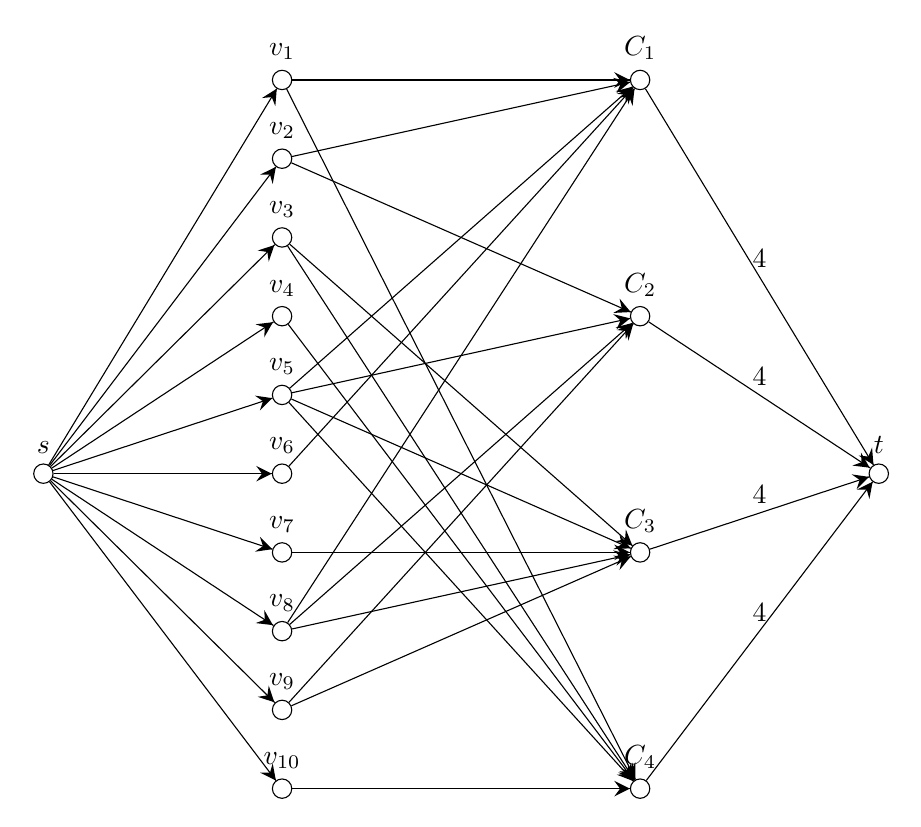
\begin{tikzpicture}[x=0.25\textwidth,
    every edge/.style={
        draw,
        postaction={decorate,
                    decoration={markings,mark=at position 1 with {\arrow[line width = 0.5mm]{stealth}}}
                   }
        }
]
\vertex (fonte) at (0,5) [label=above:$s$] {};
\vertex (v1) at (1,10) [label=above:$v_1$] {};
\vertex (v2) at (1,9) [label=above:$v_2$] {};
\vertex (v3) at (1,8) [label=above:$v_3$] {};
\vertex (v4) at (1,7) [label=above:$v_4$] {};
\vertex (v5) at (1,6) [label=above:$v_5$] {};
\vertex (v6) at (1,5) [label=above:$v_6$] {};
\vertex (v7) at (1,4) [label=above:$v_7$] {};
\vertex (v8) at (1,3) [label=above:$v_8$] {};
\vertex (v9) at (1,2) [label=above:$v_9$] {};
\vertex (v10) at (1,1) [label=above:$v_{10}$] {};
\vertex (C1) at (2.5,10) [label=above:$C_1$] {};
\vertex (C2) at (2.5,7) [label=above:$C_2$] {};
\vertex (C3) at (2.5,4) [label=above:$C_3$] {};
\vertex (C4) at (2.5,1) [label=above:$C_4$] {};
\vertex (dreno) at (3.5,5) [label=above:$t$] {};
\path
(fonte) edge (v1)
(fonte) edge (v2)
(fonte) edge (v3)
(fonte) edge (v4)
(fonte) edge (v5)
(fonte) edge (v6)
(fonte) edge (v7)
(fonte) edge (v8)
(fonte) edge (v9)
(fonte) edge (v10)
(v1) edge (C1)
(v1) edge (C4)
(v2) edge (C1)
(v2) edge (C2)
(v3) edge (C3)
(v3) edge (C4)
(v4) edge (C4)
(v5) edge (C1)
(v5) edge (C2)
(v5) edge (C3)
(v5) edge (C4)
(v6) edge (C1)
(v7) edge (C3)
(v8) edge (C1)
(v8) edge (C2)
(v8) edge (C3)
(v9) edge (C2)
(v9) edge (C3)
(v10) edge (C4)
(C1) edge node [above] {$4$} (dreno)
(C2) edge node [above] {$4$} (dreno)
(C3) edge node [above] {$4$} (dreno)
(C4) edge node [above] {$4$} (dreno)
;
\end{tikzpicture}\]

\begin{enumerate}
\item Implementação
\label{sec-6-2-1-1}

Primeiramente, precisamos ser capazes de ler a tabela acima para
passar os valores para o nosso algoritmo.
\begin{minted}[]{python}
capacidade_por_caminhao = regras[0][1]
total_de_vasilhames = regras[2][1]
\end{minted}

\begin{minted}[]{python}
vasilhames = collections.OrderedDict()
caminhoes = []
for line in seguros[1:]:
    # Nomeando os vasilhames
    vasilhame = 'v_%s' % line[0]
    vasilhames[vasilhame] = []
    for caminhao in str(line[1]).split(','):
        nome = 'C_%s' % caminhao.strip()
        vasilhames[vasilhame].append(nome)
        if nome not in caminhoes:
            caminhoes.append(nome)
\end{minted}

Vamos usar a classe RedeDeFluxo, que definimos para a questão 7.28.

\begin{minted}[]{python}
def cria_grafo(vasilhames, caminhoes, capacidade_por_caminhao):
    G = RedeDeFluxo()
    G.novo_vertice('Fonte')
    G.novo_vertice('Dreno')

    # Criando um vertice para cada caminhao e ligando esse
    # vertice ao dreno
    for caminhao in caminhoes:
        G.novo_vertice(caminhao)
        G.nova_aresta(caminhao, 'Dreno',
                      capacidade_por_caminhao, 0)

    for vasilhame, caminhoes in vasilhames.iteritems():
        # Criando um vertice para cada vasilhame e conectando
        # a fonte a cada um dos vasilhames
        G.novo_vertice(vasilhame)
        G.nova_aresta('Fonte', vasilhame, 1, 0)

        # Conectando o vasilhame a cada caminhao que pode
        # transporta-lo
        for caminhao in caminhoes:
            G.nova_aresta(vasilhame, caminhao, 1, 0)

    return G
\end{minted}

Como nesse problema as demandas já são 0, podemos aplicar
Ford-Fulkerson diretamente, usando a mesma implementação que fizemos
para o exercício 7.28.

Podemos então rodar Ford-Fulkerson e ver se o fluxo máximo encontrado
é igual ao total de vasilhames. Se for, isso significa que o problema
tem uma solução, que vamos retornar. Caso contrário não existe arranjo
possível.
\begin{minted}[]{python}
G = cria_grafo(vasilhames, caminhoes, capacidade_por_caminhao)
fluxo = G.fluxo_maximo('Fonte', 'Dreno')
if fluxo == total_de_vasilhames:
    tabela_de_vasilhames = []
    for vasilhame in vasilhames:
        for w in G.adj[vasilhame]:
            if G.fluxo[w] == 1:
                tabela_de_vasilhames.append([w.origem, w.destino])
    return tabela_de_vasilhames
else:
    return 'Impossivel'
\end{minted}

A solução para a nossa entrada:
\begin{center}
\begin{tabular}{ll}
v$_{\text{1}}$ & C$_{\text{4}}$\\
v$_{\text{2}}$ & C$_{\text{2}}$\\
v$_{\text{3}}$ & C$_{\text{3}}$\\
v$_{\text{4}}$ & C$_{\text{4}}$\\
v$_{\text{5}}$ & C$_{\text{1}}$\\
v$_{\text{6}}$ & C$_{\text{1}}$\\
v$_{\text{7}}$ & C$_{\text{3}}$\\
v$_{\text{8}}$ & C$_{\text{1}}$\\
v$_{\text{9}}$ & C$_{\text{2}}$\\
v$_{\text{10}}$ & C$_{\text{4}}$\\
\end{tabular}
\end{center}

\item Complexidade
\label{sec-6-2-1-2}

Como vimos no exercício 7.28, O algoritmo de Ford-Fulkerson tem
complexidade $O((V + E)F)$ em que $V$ é a quantidade de vértices, $E$
é a quantidade de arestas e $F$ é o maior valor possível para o fluxo.

No caso, $V = m + n + 2$, $E \leq n + nm + m$ e o maior fluxo possível é
$n$, totalizando uma complexidade máxima $O(n^2m)$, o que é polinomial na
entrada.
\end{enumerate}

\subsection{Item B}
\label{sec-6-3}

Vamos mostrar que é possível reduzir uma instância do 3-SAT a um
problema de colocar vasilhames em caminhões seguindo as restrições do
enunciado. De modo que, como 3-SAT é NP-completo, nosso problema
também é.

\subsubsection{Definindo 3-SAT}
\label{sec-6-3-1}

3-SAT é o problema de dado um conjunto de variáveis $v_1, \ldots, v_x$
e cláusulas $K_1, \ldots, K_y$, onde cada cláusula é constituída de no
máximo três elementos do universo de \textit{literais}, $\{v_1,
\overline{v_1}, \ldots, v_x, \overline{v_x}\}$, encontrar uma
atribuição de valores Verdadeiro/Falso para cada variável
que faça com que todas as cláusulas sejam verdadeiras.

\subsubsection{3-SAT $\to$ Caminhões}
\label{sec-6-3-2}

Dada uma instância do 3-SAT, vamos construir uma instância do problema
enunciado que admite solução se e somente se tal
instância do 3-SAT admite solução.

Primeiramente, note que podemos assumir que nosso
problema de 3-SAT tem pelo menos quatro variáveis, adicionando
variáveis que não aparecem em cláusula alguma se necessário.

\begin{enumerate}
\item Construção
\label{sec-6-3-2-1}

Vamos começar a construção sem as cláusulas:

\begin{itemize}
\item São $x+1$ caminhões, cada um de capacidade $3x+y$

\item Existe um vasilhame para cada um dos $2x$ literais em $\{v_1,
  \overline{v_1}, \ldots, v_x, \overline{v_x}\}$. Esses vasilhames têm o
mesmo nome do literal a que correspondem.

\item Existe um vasilhame adicional $w_i$ para cada variável $v_i$
\end{itemize}

Queremos criar restrições entre os vasilhames de modo que, em uma
atribuição válida:

\begin{enumerate}
\item $x$ dos caminhões contenham exatamente um literal verdadeiro cada.
\item O caminhão restante contenha todos os literais falsos;
\end{enumerate}

Para garantir as condições acima, vamos criar os seguintes conflitos:
\begin{itemize}
\item $w_i$ conflita com $w_j$ para todo $i \neq j$.
\item $w_i$ e conflita com $v_j$ e com $\overline{v_j}$, se $i \neq j$.
\item $v_i$ conflita com $\overline{v_i}$.
\end{itemize}

Com isso, garantimos as seguintes propriedades:

\begin{enumerate}[($P_1$)]
\item Como todos os $w_i$ conflitam entre si, é necessário um
caminhão por $w_i$.

\item Como $w_i$ conflita com todos os literais tais que
$i \neq j$, o caminhão que contém $w_i$ só pode conter literais
correspondentes a $i$-ésima variável.

\item $v_i$ e $\overline{v_i}$ não
podem estar ambas no caminhão do $w_i$, pois elas conflitam entre si.

\item Mais ainda, $\textit{exatamente}$ um elemento do par $\{v_i,
\overline{v_i}\}$ está no caminhão do $w_i$ numa atribuição válida: Se
nenhuma delas estivesse no caminhão do $w_i$, estariam ambas no único
caminhão que não contém nenhum $w$ (pois todos os outros caminhões
contém um $w_j$ com $i \neq j$, o que conflita com $v_i$ e
$\overline{v_i}$ por $P_2$), o que também não pode acontecer por $P_3$.
\end{enumerate}



Agora, vamos adicionar as cláusulas à nossa construção:

\begin{itemize}
\item Existe um vasilhame para cada uma das $y$ cláusulas $K_1, \ldots, K_y$
\end{itemize}

Com seguinte conflito:

\begin{itemize}
\item $K_i$ conflita com $v_j$ se $v_j \not\in K_i$. Similarlmente, $K_i$
  conflita com $\overline{v_j}$ se $\overline{v_j} \not\in K_i$.
\end{itemize}

Ou seja, permitimos colocar o vasilhame da cláusula $K_i$ num caminhão
apenas se a cláusula contém todos os literais que vão viajar no
caminhão.

Dessa forma, uma cláusula nunca pode viajar no caminhão dos literais
falsos, pois cada a cláusula contém no máximo três literais e temos no
mínimo quatro literais falsos, de modo que há garantidamente um
literal que não aparece na cláusula e portanto conflita com ela.

\item Obtendo uma solução
\label{sec-6-3-2-2}

Para completar a nossa redução, precisamos de duas coisas:
\begin{itemize}
\item A partir de uma solução do problema dos caminhões que construimos,
encontrar em tempo polinomial uma solução do 3-SAT correspondente
\item Provar que quando nenhuma solução do problema dos caminhões existe o
3-SAT também não tem solução
\end{itemize}

\begin{enumerate}
\item Solução caminhões $\to$ Solução 3-SAT
\label{sec-6-3-2-2-1}

Se existe uma solução para o problema, então todo caminhão que contém
um vasilhame do tipo $w_i$ também contém um vasilhame correspondente a
um literal, pela propriedade $P_4$; esse literal será marcado como
verdadeiro. Todos os outros literais serão marcados como falsos. Essa
marcação é consistente, pois para cada $i \in \{1, 2, \ldots, x\}$
exatamente um literal entre $v_i, \overline{v_i}$ que está no mesmo
caminhão que $w_i$. Como todas as cláusulas têm que estar em um
caminhão que contém um vasilhame do tipo $w_i$ e esse caminhão tem que
conter um literal que está na cláusula, essa marcação faz com que
todas as cláusulas sejam verdadeiras.


\item $\not \exists$ solução caminhões $\Rightarrow \not \exists$ solução 3-SAT
\label{sec-6-3-2-2-2}

É mais fácil provar a contrapositiva, isso é, $\exists$ solução 3-SAT
$\Rightarrow \exists$ solução caminhões.

Seja $S$ os conjuntos dos literais verdadeiros na solução do 3-SAT.
Então:
\begin{itemize}
\item $S \subset \{v_1,\overline{v_1}, \ldots, v_x, \overline{v_x}\}$
\item $\forall \; 1\leq i \leq x, |S\cap\{v_i, \overline{v_i}\}| = 1$
\item $\forall \; 1\leq j \leq y, S\cap K_j \neq \emptyset$
\end{itemize}

Podemos construir uma solução válida para o problema dos caminhões da
seguinte forma:
\begin{itemize}
\item $\forall \; 1\leq i \leq x$, coloque o vasilhame $w_i$ no caminhão $C_i$
\item $\forall \; 1\leq i \leq x$, coloque o vasilhame $S\cap\{v_i, \overline{v_i}\}$ em $C_i$
\item $\forall \; 1\leq j \leq y$, seja $i$ o menor valor tal que $v_i$ ou
$\overline{v_i}$ está em $S\cap K_j$. Coloque o vasilhame $K_j$ em $C_i$.
\item Coloque todos os literais em $\{v_1,\overline{v_1}, \ldots, v_x,
  \overline{v_x}\} - S$ no caminhão $C_{x+1}$
\end{itemize}


Isso respeita todas as restrições. De fato, cada $K_j$ está num
caminhão que só contém um vasilhame correspondente a um literal e,
pelo item 3, o vasilhame do literal não conflita com o vasilhame da
cláusula. Além disso, cada $w_i$ está em seu próprio caminhão, nenhum
par $\{v_i, \overline{v_i}\}$ aparece num mesmo caminhão e nenhum
$w_i$ aparece no mesmo caminhão de um literal $v_j$ ou
$\overline{v_j}$ com $i \neq j$.
\end{enumerate}
\end{enumerate}
% Emacs 24.4.1 (Org mode 8.2.10)
\end{document}
